%\selectlanguage{english}
\chapter*{Publicaciones}
\label{cap:publicaciones}
\addcontentsline{toc}{chapter}{\protect{Publicaciones}}

\markboth{Publicaciones}{Publicaciones}

\noindent
A continuaci�n se expone una lista de los trabajos que han sido publicados como resultado de la investigaci�n llevada a cabo a lo largo de esta tesis doctoral. Estas publicaciones avalan el trabajo realizado poniendo de manifiesto tanto su inter�s como su validez cient�fica.\\

\begin{Large}
Revistas
\end{Large}

\begin{enumerate}
	\item Fernando Benito-Picazo, Pablo Cordero, Manuel Enciso, �ngel Mora. \textit{Minimal generators, an affordable approach by means of massive computation}. The Journal of Supercomputing, Springer, 2018. 
	
	{\tt DOI: 10.1007/s11227-018-2453-z}
	
Factor de impacto en J.C.R. 2017: 1,532. Posici�n 43 de 103 (Q2) en la categor�a: `Computer Science, Theory \& Methods'.
	\item Fernando Benito-Picazo, Manuel Enciso, Carlos Rossi, Antonio Guevara. \textit{Enhancing the conversational process by using a logical closure operator in phenotypes implications}. Mathematical Methods in the Applied Sciences, John Wiley \& Sons Ltd, 2017. 
	
	{\tt DOI: 10.1002/mma.4338}
	
Factor de impacto en J.C.R. 2017: 1,18. Posici�n 91 de 252 (Q2) en la categor�a: `Mathematics, Applied'.
	\item Fernando Benito-Picazo, Pablo Cordero, Manuel Enciso, �ngel Mora. \textit{Reducing the search space by closure and simplification paradigms. A parallel key finding method}. The Journal of Supercomputing, Springer, 2016. 
	
	{\tt DOI: 10.1007/s11227-016-1622-1}
	
Factor de impacto en J.C.R. 2016: 1,349. Posici�n 52 de 104 (Q2) en la categor�a: `Computer Science, Theory \& Methods'.
\end{enumerate}

\begin{Large}
Congresos Internacionales
\end{Large}

\begin{itemize}
	\item Fernando Benito-Picazo, Pablo Cordero, Manuel Enciso, �ngel Mora. \textit{Closed sets enumeration: a logical approach}. Proceedings of the Seventeenth International Conference on Computational and Mathematical Methods in Science and Engineering, CMMSE, 2017. C�diz, Spain, July 4-8, pp. 287-292, ISBN: 978-84-617-8694-7.
	\item Fernando Benito-Picazo, Manuel Enciso, Carlos Rossi, Antonio Guevara. \textit{Conversational recommendation to avoid the cold-start problem}. Proceedings of the Sixteenth International Conference on Computational and Mathematical Methods in Science and Engineering, CMMSE, 2016. C�diz, Spain, July 4-8, pp. 184-190, ISBN: 978-84-608-6082-2.
	\item Fernando Benito-Picazo, Pablo Cordero, Manuel Enciso, �ngel Mora. \textit{Keys for the fusion of heterogeneous information}. Proceedings of the Fifteenth International Conference on Computational and Mathematical Methods in Science and Engineering, CMMSE, 2015. C�diz, Spain, July 6-10, pp. 201-211, ISBN: 978-84-617-2230-3.
	\item Fernando Benito-Picazo, Pablo Cordero, Manuel Enciso, �ngel Mora. \textit{Increasing the Efficiency of Minimal Key Enumeration Methods by Means of Parallelism}. Proceedings of the 9th International Conference on Software Engineering and Applications, ICSOFT-EA, Vienna, Austria, August 29-31, 2014, pp. 512-517.
	
	{\tt DOI: 10.5220/0005108205120517} 
\end{itemize}

\newpage
\begin{Large}
Workshops
\end{Large}

\begin{itemize}
	\item Fernando Benito-Picazo. \textit{Parallelism in the search of minimal keys from implications using tableaux methods}. Workshop: L�gica, Lenguaje e Informaci�n. Dpto. Matem�tica Aplicada. Unidad de Investigaci�n en L�gica, Lenguaje e Informaci�n, Andaluc�a Tech. Universidad de M�laga, Noviembre 2014.
\end{itemize}

\vspace{0.5cm}

\begin{figure}[htbp]
		\begin{center}
			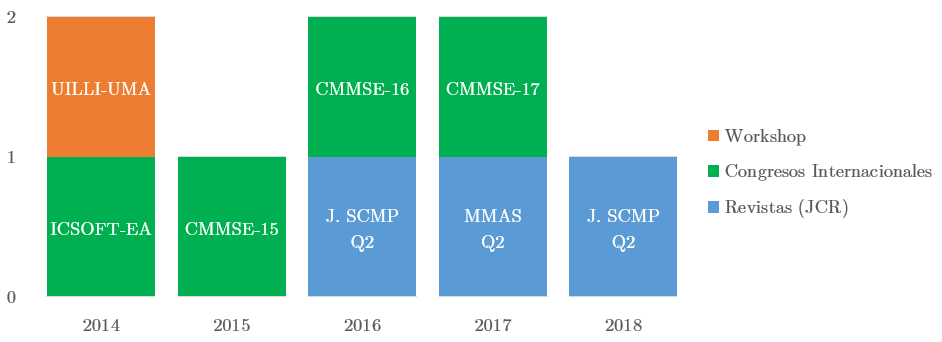
\includegraphics[height=.23\textheight,width=.95\textwidth]{graficoPublicaciones.png}
		\end{center}
		\caption{Producci�n cient�fica}
		\label{figura:graficoPublicaciones}
\end{figure}



% =====================================================================
% =====================================================================
% =====================================================================